\documentclass[conference]{IEEEtran}

%+++++++++++++++++++++++++++++++++++++++++++++++++++
\usepackage[pdftex]{graphicx}
\usepackage{svg}
\usepackage{amsmath}
\usepackage{eqparbox}
\usepackage{verbatimbox}
\usepackage[backend=biber,style=ieee,citestyle=numeric]{biblatex}
\addbibresource{references.bib}
\usepackage{hyperref}
\usepackage{booktabs,ragged2e}
\usepackage[flushleft]{threeparttable}
\usepackage{tabularx}
\renewcommand\TPTtagStyle{\textit}
%+++++++++++++++++++++++++++++++++++++++++++++++++++

\usepackage{verbatimbox}
\graphicspath{{img/}}

\newcolumntype{C}{>{\centering\arraybackslash}X} % centered version of "X" type

\begin{document}

%+++++++++++++++++++++++++++++++++++++++++++++++++++
\title{\textbf{\LARGE A Study on Convolutional Neural Networks Variant for Face Mask Classification}}
\author{\authorblockN{Yang Qixiu\authorrefmark{1}(ID 2175021167), Lu Xu\authorrefmark{1}(ID 2175122023), Sun Zihong\authorrefmark{2}(ID 2176112709),\\ Galbiati Tiberio\authorrefmark{0} (ID 3120999064), Casarico Massimo\authorrefmark{2} (ID 3120999073),\\ Muhammad Rifki Kurniawan\authorrefmark{2} (ID 3120999259), Siriporn Pattamaset\authorrefmark{2} (ID 4120999061).\\ \emph{Big Data and Deep Learning Group 39.}}
\authorblockA{\authorrefmark{1}School of Mechanical Engineering, Xi'an Jiaotong University, Xi'an, China}
\authorblockA{\authorrefmark{2}School of Electronic and Information Engineering, Xi'an Jiaotong University, Xi'an, China}}
%+++++++++++++++++++++++++++++++++++++++++++++++++++

\maketitle


% ================
% # Abstract     #
% ================

\begin{abstract}
Deep learning architectures including Convolutional Neural Networks (Convnets) have been broadly applied into diverse numbers of sectors such as surveillance due to high accuracy. Inspired by the recent situation on pandemic outbreaks and, concurrently, surveillance system application involvement in public using AI, we build Convenets architectures for binary image classification task of face mask classification. The aim of the project is to identify human face images wearing a mask and not wearing a mask. The experiments are based on a public dataset available on Kaggle that was collected combining Google searches and the CelebFace dataset. In this report we will discuss the classification performance of the different network architectures based on classification accuracy metrics, such as f1-score, and performance metrics including number of parameters. We are investigating the corollary of pre-trained networks for transfer learning as opposed to learning  from random initialization. The experiments resulted that MobileNetV2 with ImageNet pre-trained weight is considerably superior among others with the high accuracy metrics along with its lightweight parameters which sum up its capability to be deployed into mobile or edge devices. Moreover, by simply training the task on simple naive hand-crafted Convnets, we can achieve very competitive high accuracy compared to other state-of-the-art sophisticated backbone. 
\end{abstract}

\begin{keywords}
image classification, deep learning, medical face mask, transfer learning.
\end{keywords}


% ========================
% # I. Introduction      #
% ========================

\section{Introduction and theoretical background}

The COVID-19 pandemic has become global pandemic since December 2019, the country and society have advocated wearing masks to prevent infection and protect public health and safety, so testing whether people wear masks has become a new demand. Combining this with the course content, we create an algorithm that can directly detect is a person is wearing a face mask or not.





 % ================== BINARY CLASS ==================
\subsection{Problem Formulation of Binary Classification}
The image classification objective is to distinguish different categories of input images according to the semantic information of the image. It is the core of computer vision and the basis of other high-level vision tasks such as object detection, image segmentation, object tracking, behavior analysis, and face recognition. Yet binary classification means that the classification task categories is binary or having two classes.

The binary task is formally defined as the following illustration. Given $X$ is the dataset --- in this case is face-mask dataset --- containing sets of image label pairs $\left \{ \left ( x_{i},y_{i}  \right ), 1\leq i\leq N, y_{i} \in \left \{ 1,0 \right \} \right \}$ and $x_{i} \in \mathbb{R} ^ {H \times W \times C}$ where $H, W$ and $C$ denotes the image size referring height, width, and number of channels, respectively. Further we resize all the samples into height and width in the size of 224x224 with 3 number of channels for its RGB channel.  In this experiment, we propose to use off-the-shelf backbones and compare with our two hand-crafted Convnets. Therefore, the designated experimentations encompass a set of discriminative models $F$ with sigmoid $\phi(.)$ classifier outputting probability value spreading out $\left \lfloor 0,1 \right \rfloor$. 



\subsection{CNN}
Convolutional Neural Networks (CNN) are a type of feedforward neural networks that include convolution calculations and has a deep structure. They are specialized for processing data with a grid-like topology \cite{goodfellow-deep}. It is mainly composed of input layer, convolutional layer, activation function, pooling layer, fully connected layer, and loss function. Its essence is feature extraction and decision inference. 



 % ================== TRANSFER ==================
\subsection{Transfer Learning on Classification}
\label{transfer}
Transfer learning refers to the transfer of learned and trained model parameters to a new model to help new model training. Considering that most data or tasks are related, we can share the learned model parameters (knowledge learned by the model) to the new model in a certain way through transfer learning to speed up and optimize the learning efficiency of the model instead of starting from scratch.

Transfer learning is a machine learning method where a model developed for a task is reused as the starting point for a model on a second task. It is a popular approach in deep learning where pre-trained models are used as the starting point on computer vision and natural language processing tasks given the vast compute and time resources required to develop neural network models on these problems and from the huge jumps in skill that they provide on related problems. Transfer learning is the improvement of learning in a new task through the transfer of knowledge from a related task that has already been learned \cite{olivas-handbook}.

From a mathematical prospective, transfer learning can be described as follows. A domain $\mathcal D$ consisting of: a feature space $\mathcal x$ and a marginal probability distribution $P(X)$, where $X$={$x_1,x_2,...,x_n$} $\in \mathcal X$. Given a specific domain, $\mathcal D$={$\mathcal X,P(X)$}, a task consists of two components: a label space $\mathcal Y$ and an objective predictive function $f:\mathcal X \to \mathcal Y$. The function $f$ is used to predict the corresponding label $f(x)$ of a new instance $x$. This task, denoted by $\mathcal T$={$\mathcal Y,f(x)$}, is learned from the training data consisting of pairs {$x_i,y_i$}, where $x_i \in X$ and $y_i \in \mathcal Y$. Going further, given a source domain $\mathcal D_s$ and learning task $\mathcal T_s$, a target domain $\mathcal D_T$ and learning task $\mathcal T_T$, where $\mathcal D_s \neq \mathcal D_T$, or $\mathcal T_S \neq \mathcal T_T$, transfer learning aims to help improve the learning of the target predictive function $f_T()$ in $\mathcal T_T$ using the knowledge in $\mathcal D_S$ and $\mathcal T_S$.  

Is intuitive that the benefits brought from a transfer learning approach are numerous. In the above mentioned book, the authors summarise them in three main blocks: a higher start in the performance curve (the initial skill, before refining the model, on the source model is higher than it otherwise would be), a higher slope (the rate of improvement of skill during training of the source model is steeper than it otherwise would be) and a higher maximum possible performance (the converged skill of the trained model is better than it otherwise would be).

To practically demonstrate the above mentioned advantages, Kafeng Wang et al.,\cite{Wang2020PayAT} compared transfer learning to traditional compression methods and stated  how transfer learning offers the chance for CNNs to learn with limited data samples by transferring knowledge from models pre-trained on large datasets. Transfer learning methodology not only is capable to determine a new model with a higher target task accuracy, but also further accelerates it by computing a subset of channel neurons in each convolutional layers and under a wide range of datasets, the smallest drop in validation accuracy under the same speed-up constraints when compared to traditional compression methods.


\subsection{ Deep Learning Frameworks}
In order to improve work efficiency, researchers wrote codes into a framework and put them on the Internet for all researchers to use together. The most popular deep learning frameworks in the world are PaddlePaddle, Tensorflow, Caffe, Theano, MXNet, Torch and PyTorch. 

In this project we implement the deep learning models using TensorFlow, Keras, and PyTorch. 

Google's open source Tensorflow is an open source mathematical calculation software developed in C++ language. It uses the form of Data Flow Graph to perform calculations. It is the most widely used framework in the world and has the largest community. 

Keras is a deep learning API written in Python, running on top of the machine learning platform TensorFlow. It was developed with focus on enabling fast experimentation.

PyTorch is developed by the Torch team and is a Python-first deep learning framework. Its predecessor was Torch, but PyTorch is more flexible, supports dynamic graphs, and provides a Python interface. 

 


\section{Related Works}
\textbf{Face mask classification}. The related studies of face mask classification are predominated by approaches using deep learning, especially Convnets architecture. Generally the study can be categorized into two different tasks: classification \cite{Loey2020AHD, Chowdary2020FaceMD, Sanjaya2020} and  detection task\cite{Jiang2020, Qin2020, Loey2020FightingAC, Chavda2020, Suresh2021, Roy2020}. In \cite{Chowdary2020FaceMD} was adopted a pre-trained backbone of InceptionV3 with additional both convnets  and multi-layer perceptrons for the head classifier while involving 8-variants data augmentations as oversampling strategy to alleviate imbalance dataset distribution. While \cite{Loey2020AHD} proposed a similar strategy but exploited ResNet18 features extractor along with attached classifier composing SVM, decision tree, and the ensemble. However, neither of them deeply take the computational cost and complexity of the architecture into consideration even as application study requires comprehensive performance metrics due to potentially hardware limits and energy consumption such as on the edge deployment. 

\textbf{Face mask detection}. Contrarily face mask detection goes beyond classification that directs subsequent face localization and classification either wearing mask or not. Therefore given input images the model designates to predict bounding boxes with respect to the objects and determine associated correct labels for each predicted bounding box. Recently, the utilization of pre-trained network alongside developing on-top-of off-the-shelf state-of-the-art object detection framework such as  one-stage framework comprises YOLO\cite{Redmon2016YouOL} and its variants \cite{Redmon2018YOLOv3AI} and SSD\cite{Liu2016SSDSS} or two-stage approach resembling Faster R-CNN\cite{Ren2015FasterRT}. Among those is \cite{Loey2020FightingAC} that developed a mask detector constructed around YOLOv2 but replacing the darknet backbone with pre-trained ResNet50 which benefited by skip-connections to create more useful representation for YOLOv2 localizer. In contrast, \cite{Qin2020} introduced SRCNet assembled from a super-resolution module as input quality enhancer before forwarded into the classifier. The super-resolution module will restore image details from low-resolution images so as the classifier gets restored inputs which significantly improve accuracy on low quality images. While the feature pyramid network was proposed by \cite{Jiang2020} for enriching the output semantic features by concatenating multiple-level feature maps for the detector inputs. This is resulting in comparable improvement on accuracy metrics relative to the baseline.

\textbf{Transfer learning}. The training regime via transfer learning or so called knowledge transfer appeared to be standard trick in deep learning application. This allows to transfer knowledge either from different or related domain, tasks, and distributions between the source and target \cite{Pan2010ASO, Torrey2009Chapter1T}. Predominantly, the source domain for computer vision task is using natural images belonging to ImageNet\cite{5206848} dataset for creating pre-trained model. While the standard techniques in transfer learning for visual task branched into two which include "fixed-feature transfer" --- freezing the backbone and replace the classifier with task-specific networks --- and "full-network transfer"\cite{Salman2020DoAR} --- fine-tuning the whole networks. Early study on transfer learning employed dimensionality reduction to construct latent features as a proxy for connecting the source with target latent features thru minimizing the distance in this latent space\cite{Pan2008}. Yosinski et al., \cite{Yosinski2014HowTA}, examine the transferability of pre-trained neural networks which deduced that transferability declines as the domain gap between source and target task is high. But, weight initialization from pre-trained resulted in better generalization and accuracy than initializing randomly. Later, layer-wise transferability features problem is resolved via Deep Adaptation Network (DAN) by \cite{DBLP:conf/icml/LongC0J15} with projecting those into kernel Hilbert space and diminishing between domains inconsistency. While, \cite{Kornblith2019DoBI} studied comprehensively the correlation of the performance of ImangeNet pre-trained on the downstream task and found that training regime such as regularization used is susceptible to downgrading the downstream task and not overly beneficial for fine-grained tasks.

\section{Proposed Method}

\subsection{Introduction to The Face Mask Data Set}

This dataset comprises facial images of people wearing face mask and not wearing face mask for classification purpose. The original data set was already split into training set of 10,000 samples, test  of 992 samples and validation of 800 samples. The dataset consists of almost 12,000 images for a total of  328.92MB in size. The images have a minimum size of 25 pixels and a maximum of 563 pixels. The majority length/width is 224 (224 x 224 x 3) pixels as shown in Fig 1. The original dataset can be downloaded from Kaggle (\url{https://www.kaggle.com/ashishjangra27/face-mask-12k-images-dataset}).


\begin{figure}[ht!] %!t
\centering
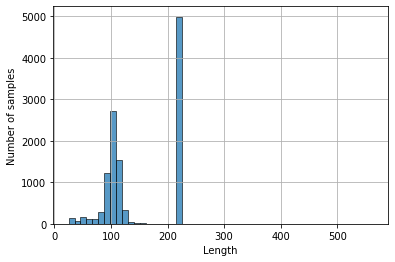
\includegraphics[width=2.8in]{size.png}
\caption{ The distribution of the length of the images in the dataset.}
\label{bench}
\end{figure}

In classification task, the dataset should have balance in the number of instances of each class in order to reduce the bias towards the majority class and prevent false positive and false negative classifications. This data set was already well balanced when splitted into training set, testing set, validation set as shown in Fig 2.

\begin{figure}[ht!] %!t
\centering
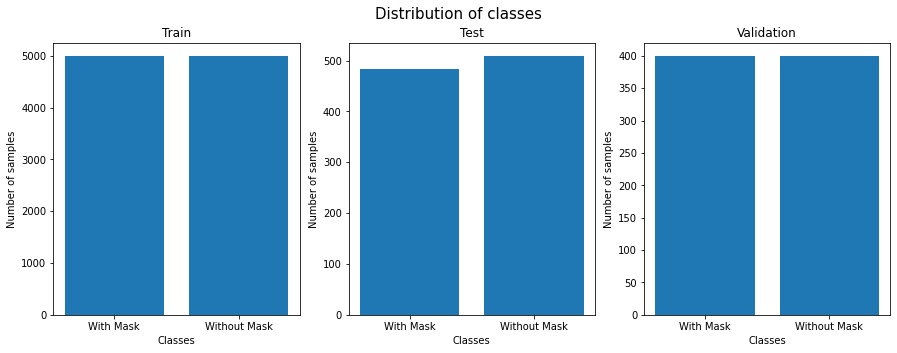
\includegraphics[width=3.4in]{distribution.png}
\caption{ Class distribution of the dataset.}
\label{bench}
\end{figure}

\subsection{Features Transfer in Binary Classification}
Binary classification task aims to predict the label $\hat{y_{i}}$ given input $x_{i}$ with $\hat{y_{i}} \in \left \{ 0,1 \right \}$. Let the $\theta_{p}$ denotes the pre-trained weight from the ImageNet pre-trained model for features extraction. We used this pre-trained weight as initialization of the model $f(.;\theta_{p})$ while training on the batches of the dataset. While in this experiment, we did not freeze the features extractor and let the training steps fine-tune the weight of both features extractor and the classifier. Then, we has an objective to minimize the loss value to obtained best parameters $\theta$ given given image-label pairs in a batch approximately equivalent to dataset distribution $D$  

\begin{equation}
    \min_{\theta} \mathbb{E}_{\left ( x,y \right ) \sim  D} \left [ \mathcal{L}_{BCE} \left ( f(x;\theta), y \right ) \right ]
\end{equation}
. In this context, we employ binary cross entropy loss $\mathcal{L}_{BCE}$ which measure the binary cross entropy between the target $y$ and the output $f(x)$ as following equation
Eq.(\ref{eqn:binaryloss}) which the gradient with respect to this loss will be used as the learning projection in parameters space 

\begin{equation}
\label{eqn:binaryloss}
\mathcal{L}_{BCE}=-\frac{1}{N} \sum_{i=1}^{N} y_{i} \cdot \log \left(f\left(x_{i}\right)\right)+\left(1-y_{i}\right) \cdot \log \left(1-f\left(x_{i}\right)\right)
\end{equation}.

\subsection{Architectures Variation}

\subsubsection{Hand-craft CNN}
In this report, we proposed two CNN-based models for face mask detection with different architectures that will be explained in detail in the experiment section.

\subsubsection{EfficientNet}
EfficientNet is a group of convolutional neural network models consisting of eight models from B0 to B7, with each subsequent model number referring to variants with more parameters and higher accuracy. EfficientNet model architecture will have to scale in three stages: (I) Depthwise Convolution and Pointwise Convolution, (II)Inverse ResNet blocks consisting of a layer that squeezes the channels, then a layer that extends the channels and (III) Linear bottleneck that uses linear activation to prevent loss of information from ReLU.\cite{DBLP:journals/corr/abs-1905-11946}

\subsubsection{ResNet}
The deeper the shallow CNN network, the better the effect, but increasing the number of layers after reaching a certain depth will cause the network to converge more slowly and the accuracy rate becomes worse. To solve this problem, the ResNET was born.The basic idea of ResNet is to introduce a "shortcut connection" that can skip one or more layers to improve performance.

\subsubsection{Xception}%done!
Xception stands for \textit{Extreme version of Inception}, it is a convolutional neural network architecture that relies solely on depthwise separable convolution layers.
A depthwise separable convolution splits a kernel into 2 separate ones that do two convolutions: 
\begin{enumerate}
    \item Depthwise Convolution \\
    This module deals not just with the spatial dimensions, but also with the depth dimension (n. of channels) because the spatial convolution is performed independently over each channel of the input.
    \item Pointwise Convolution \\
    This is so named because it uses a 1x1 kernel, projecting the channels output by the depthwise convolution onto a new channel space. In short, the Xception architecture is a linear stack of depthwise separable convolution layers with residual connections. Xception architecture has overperformed VGG-16, ResNet and Inception V3 in most classical classification challenges \cite{xception}.
\end{enumerate}

\subsubsection{MobileNetV2} 
Improved version of mobile architecture developed by Google Research \cite{Sandler2018MobileNetV2IR}, MobileNetV2 is a multi-task-purpose state-of-the-art backbone specialized for mobile devices. This architecture is built on top of three essential components named inverted residual block, lightweight depthwise separable convolutional layer, and linear bottlenecks. Additionally, some tricks are used for accuracy improvement including chop off the non-linearity in narrow layers as the effort to build better features representation thru preserving the information. The originated research has proven that this architecture is applicable for various visual tasks such as object detection or object segmentation.  

\subsubsection{MnasNet}
Designed specifically for mobile device deployment, MnasNet\cite{Tan2019MnasNetPN} is developed by a similar group who founded MobileNet. The networks structure was developed via neural architecture search that directly incorporated the performance metrics such as model latency into the searching algorithm objective function. Thereby the NAS algorithm will find out the best architecture by optimizing the trade-off between structure complexity and performance in terms of latency. However, instead of using common FLOPS as metrics performance, MnasNet measure the performance as respects to real-world inference latency of the model deployed on mobile phones.




% ==========================
% # III. Experiments #
% ==========================
\section{Experiments}
Colaboratory is a Google research project created to help disseminate machine learning education and research. It is a free cloud service and supports free GPU . It's a Jupyter notebook environment that requires no setup to use and runs entirely in the cloud.

In this experiments, we jointly write and run the code on the colab platform, we created different models based on the same dataset, but using different architectures and hyperparameters as shown in Table\ref{T1} and we compared them. Because we do not have access to high GPU computation resource in order to do grid search. The experimental models consist of two CNN hand-craft models and transfer learning with pre-trained models which are EfficientNetB0, Xception, ResNet18, MobilenetV2, and MnasNet. We also added image augmentation to the data generator as follows: horizontal flip 10 degree, rescale to 1/255, and image normalization. 

\begin{table}[h]\centering
%\small\sf
\caption{The summary of parameters setup in each experiments.}\label{T1}
\begin{tabularx}{\linewidth}{l l l l l l}
\toprule
Model&Image shape&batch size&Learning rate\\
\midrule
Hand-craft CNN1&(224x224x3)&32&0.0003\\
Hand-craft CNN2&(256x256x3)&64& 0.0004\\
EfficientNetB0&(224x224x3)&16& 0.00001\\
ResNet18&(224x224x3)&32& 0.001\\
Xception&(256x256x3)&64& 0.001\\
\bottomrule
\end{tabularx}
\end{table}

% =========
% # model1 #

\subsection{Model 1 : Hand-craft CNN1}
\subsubsection{Architecture}
Hand-craft CNN1 is a hand-craft model with 3 convolutional layers as shown in Fig.3. The model was created as follows:
\begin{itemize}
    \item The input shape is 224x224 as the majority image shape of the image dataset. The first layer uses 32 filters with kernel size of (3 × 3) and stride of 1.
    \item Next, rectified linear activation function (ReLU) layer, batch normalization layer was added with 0.90 momentum, and add a max pooling layer which uses a pool size of 2, and then add dropout with 0.2.
    \item Then,we repeat for 2 times the structure of convolutional layers followed by ReLU activation function layer, batch normalization layer and a max pooling layer. The number of output filters started from 32, 64, 128, and 128. 
    \item Lastly, flatten the input, and add 3 Dense layers and batch normalization layer, and sigmoid activation function layer.
    The model architecture is shown in Fig.3.
    
\end{itemize}

\begin{figure}[ht!] %!t
\centering
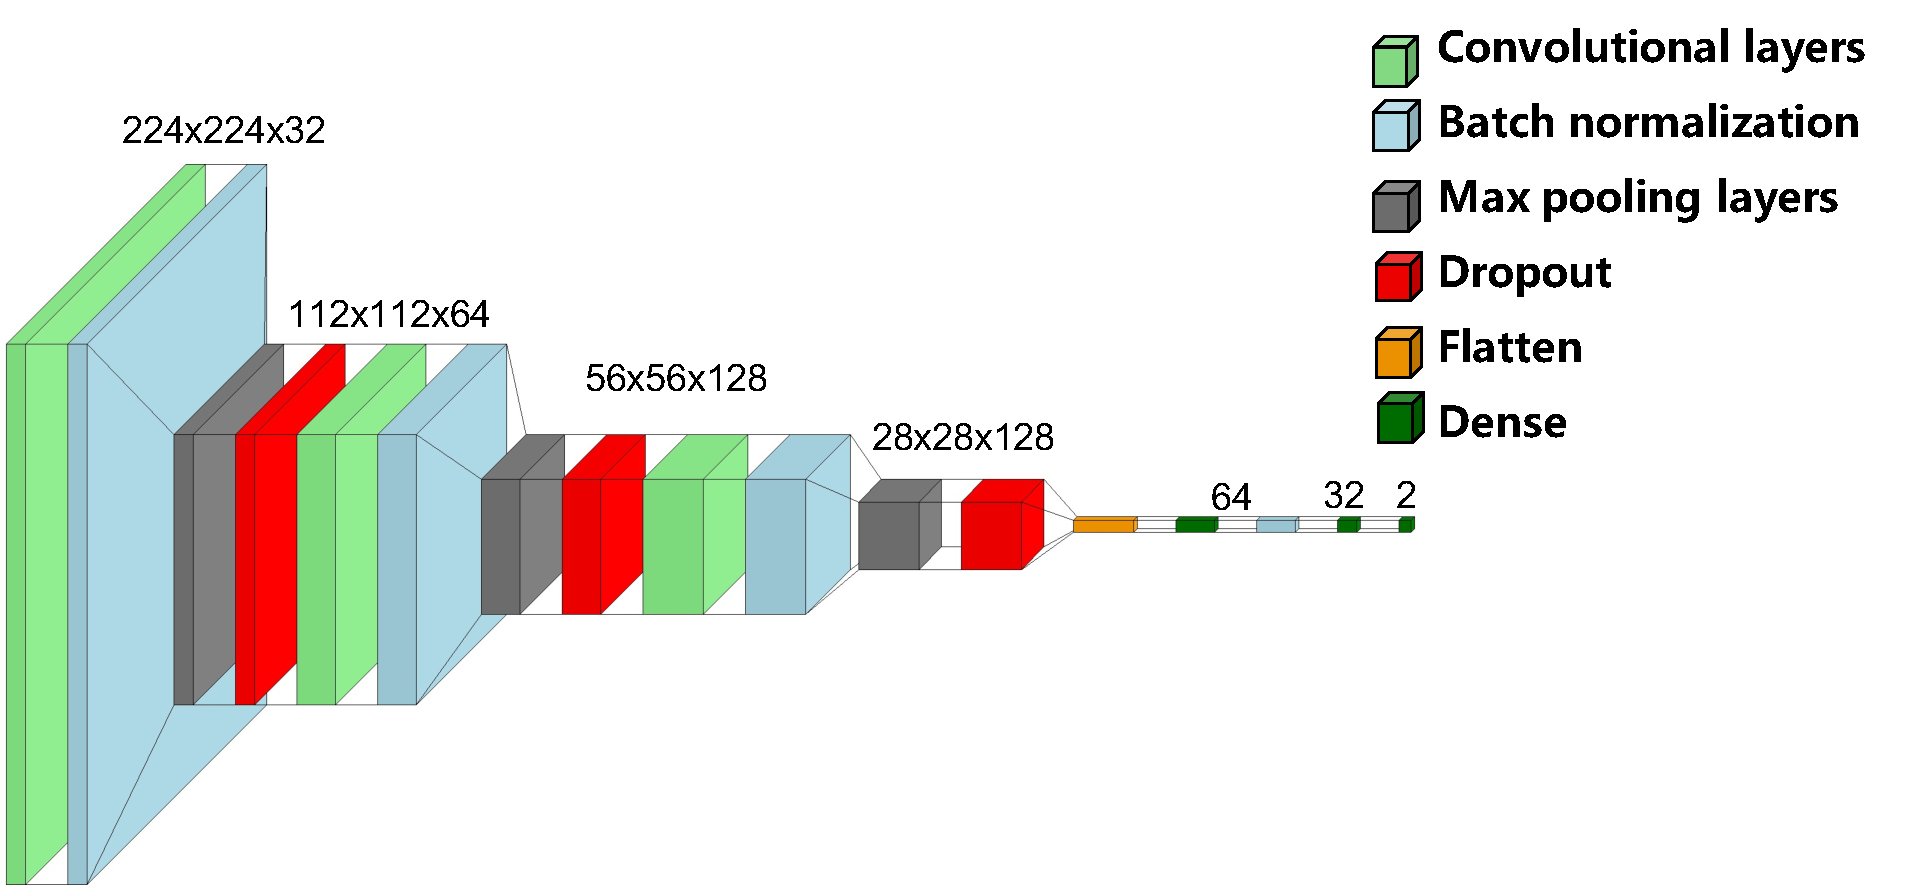
\includegraphics[width=3.5in]{CNN1.pdf}
\caption{ Hand-craft CNN1 architecture}
\label{bench}
\end{figure}

\subsubsection{Hyperparamters Tuning}
\begin{itemize}
    \item Loss function as Binary Crossentropy.
    \item The learning rate is $3\times10^{-4}$.
    \item Using Adam optimizer as the optimizer for training. 
    \item The early stop method was used to prevent overfitting during training with \texttt{patience = 5}.
\end{itemize}


\subsubsection{Evaluation Metrics}
The accuracy and loss are considered as the evaluation metrics.

% =========
% # model2 #

\subsection{Model 2 : Hand-craft CNN2}
\subsubsection{Architecture}
Hand-craft CNN2 was created using a custom architecture as shown in Fig.4, based on \cite{hands-on}\\
Here follows the description of the layers added:
\begin{itemize}
    \item The layer uses 64 fairly large filters (7 × 7) with stride equal to 1 because  the input images are not so small. Here we set the input shape to 256x256, this could be changed to fit better the distribution of the images of the set, but as we will see later, this value does not make big differences.
    \item Then we add another convolution layer, similar to the one above but with smaller filters, and without stride.
    \item Next we have a max pooling layer which uses a pool size of 2, so it divides each spatial dimension by a factor of 2.
    \item Then we repeat for 3 times the structure of two convolutional layers followed by a max pooling layer. The value 3 is a hyperparameter which can be tuned. It is important to note that the number of filters grows as we climb up the CNN toward the output layer, we started from 64, then 128, 256, 512. 
    \item We finally flatten the input, and add 3 Dense layers. Since we are using binary classification the last activation is sigmoid.
    
\end{itemize}

\begin{figure}[ht!] %!t
\centering
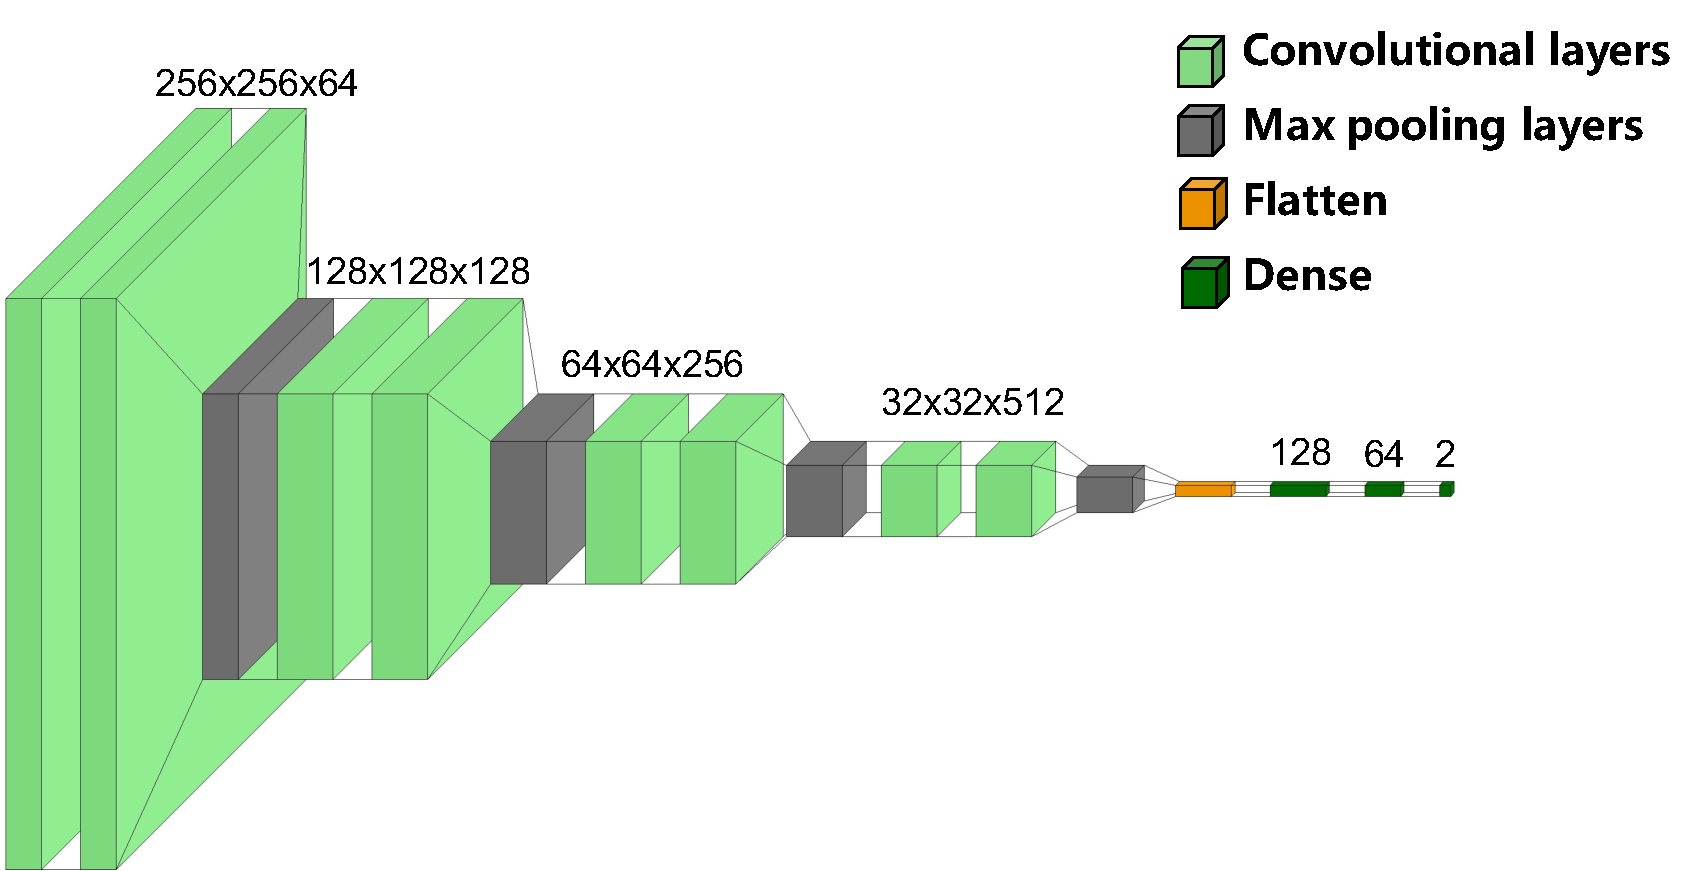
\includegraphics[width=2.8in]{CNN2.pdf}
\caption{ Hand-craft CNN2 architecture}
\label{bench}
\end{figure}

In Table\ref{table:mod1-arch} is reported the full layer architecture for the model 2.
\begin{table}[ht!] %!t
\centering
\caption{Layer Architecture}
\begin{verbnobox}[\fontsize{8pt}{8pt}\selectfont]
Model: "sequential"
________________________________________________
Layer           Output Shape           Param #   
================================================
conv2d         (None, 256, 256, 64)    9472      
________________________________________________
conv2d_1       (None, 256, 256, 64)    36928     
________________________________________________
max_pooling2d  (None, 128, 128, 64)    0         
________________________________________________
conv2d_2       (None, 128, 128, 128)   73856     
________________________________________________
conv2d_3       (None, 128, 128, 128)   147584    
________________________________________________
max_pool2d_1   (None, 64, 64, 128)     0         
________________________________________________
conv2d_4       (None, 64, 64, 256)     295168    
________________________________________________
conv2d_5       (None, 64, 64, 256)     590080    
________________________________________________
max_pool2d_2   (None, 32, 32, 256)     0         
________________________________________________
conv2d_6       (None, 32, 32, 512)     1180160   
________________________________________________
conv2d_7       (None, 32, 32, 512)     2359808   
________________________________________________
max_pool2d_3.  (None, 16, 16, 512)     0         
________________________________________________
flatten        (None, 131072)          0         
________________________________________________
dense          (None, 128)             16777344  
________________________________________________
dense_1        (None, 64)              8256      
________________________________________________
dense_2        (None, 2)               130       
================================================
Total params: 21,478,786
Trainable params: 21,478,786
Non-trainable params: 0
\end{verbnobox}
\label{table:mod1-arch}
\end{table}

\subsubsection{Hyperparamters Tuning}
\begin{itemize}
    \item Since we are doing binary classification we choose \textit{Binary Crossentropy} as Loss function.
    \item For learning rate we used $1E-4$
    \item As optimizer we used \textit{Adam} optimization, which is a momentum optimizer, so it uses an exponentially decaying average for past gradients but in addition it also keeps track of the decaying average for past squared gradients. 
    \item In order to avoid overfitting we used the early stop method setting \texttt{patience = 5}
\end{itemize}



\subsection{Model 3: Transfer learning with EfficientNetB0}
We utilized EfficientNetB0\cite{DBLP:journals/corr/abs-1905-11946}  which is the pre-trained ImageNet model. EfficientNet is built for ImageNet classification contains 1,000 classes.
\subsubsection{Architecture}
This model used EfficientNetB0 as base model made available in Keras applications. To apply this pre-trained model to our purpose, we modified classifier from 1,000 classes to 2 classes by attaching fully connected layer. In the experiment, we tried both pre-trained weights and random weights.

\subsubsection{Hyperparamters Tuning}
\begin{itemize}
    \item Loss function as Binary Crossentropy.
    \item The learning rate is $1\times10^{-5}$.
    \item Using Adam optimizer as the optimizer for training. 
    \item The early stop method was used to prevent overfitting during training with \texttt{patience = 5}.
\end{itemize}

\subsubsection{Evaluation Metrics}
The accuracy and loss are considered as the evaluation metrics.


\subsection{Model 4: Transfer learning with ResNet18, Mnasnet, and MobileNetV2}
\subsubsection{Architecture} The model weight was initialized from Imagenet pre-trained model and then fine-tune the model into down-stream face-mask dataset. The model was implemented on top of PytorchLightning and was trained on single GPU.
\subsubsection{Hyperparamters Tuning}
\begin{itemize}
    \item Loss function as Binary Crossentropy.
    \item The learning rate is $1\times10^{-3}$.
    \item Using Adam optimizer as the optimizer for training. 
    \item number of epochs 20.
    \item weight decay is 0.0005.
\end{itemize}

\subsection{Model 5 : Xception with transfer learning}
This fifth model is still implemented with Tensorflow, but this time we used transfer learning as explained in Section \ref{transfer}.
We used Xception and to reach the highest score we did some hyperparameters tuning. The parameters we tuned were the learning rate, the batch size, the number and dimension of Dense layers and the patience for early stopping callback.
Initially we didn't use Dense layer, but we then notice that adding Dense layers we were able to reduce the gap between training accuracy and validation accuracy.

We tested different version of transfer learning with Xception:
\begin{itemize}
    \item Cross validation
    \item Using two consecutive trainings: one with frozen base model and the other with the whole model unfrozen
    \item Callback to control the variation of learning rate
\end{itemize}

\subsubsection{Architecture}
We used Xception as base model and we then attach fully connected layers.
We find out that doing two consecutive trainings (one with base model frozen 
and the other with model unfrozen) didn't make much difference in Xception.
In the end we made only one training with the model unfrozen to speed up
the training time.

\subsubsection{Evaluation Metrics}
The accuracy and loss are considered as the evaluation metrics.
\begin{table*}[h]
\begin{threeparttable}
\caption{Accuracy and Performance Benchmark on Various Networks Architectures}
\label{tab:2}
\setlength\tabcolsep{0pt} % make LaTeX figure out intercolumn spacing

\begin{tabularx}{\textwidth}{@{}l*{6}{C}c@{}}
\toprule
     Architecture & Weight Initialization & 
     \multicolumn{4}{c}{Accuracy (\%)} & 
     \multicolumn{1}{c}{Performance} \\
\cmidrule{3-7}
     & & Acc & Precision & Recall & F1-Score & Parameters (Millions) \\
\midrule
     Hand-craft1 & random & 99.3 & 99.3 & 99.3 & 99.3 & 6.5 \\
     Hand-craft2 & random & 99.1 & 99.1 & 99.1 & 99.1 & 19.4  \\
     ResNet18 \cite{He2016DeepRL} & random & 98.9 & 98.8 & 99.2 & 99.0 & 11.2 \\
     ResNet18 \cite{He2016DeepRL} & pretrained & 99.2 & 98.6 & 100.0 & 99.3 & 11.2  \\
     Xception \cite{xception} & pretrained & 99.4 & 99.4 & 99.4 & 99.4 & 22.3  \\
     MobilenetV2 \cite{Sandler2018MobileNetV2IR} & random & 99.2 & 98.6 & 100.0 & 99.3 & 2.2  \\
     MobilenetV2 \cite{Sandler2018MobileNetV2IR} & pretrained & 99.7 & 100.0 & 99.6 & 99.8 & 2.2 \\
     Efficientnetb0 \cite{DBLP:journals/corr/abs-1905-11946} & random & 99.5 & 99.2 & 100.0 & 99.6 & 4.0 \\
     Efficientnetb0 \cite{DBLP:journals/corr/abs-1905-11946} & pretrained & 99.4 & 99.0 & 100.0 & 99.5 & 4.0 \\
     MnasNet \cite{Tan2019MnasNetPN} & random & 98.6 & 98.8 & 98.6 & 98.7 & 3.1 \\
     MnasNet \cite{Tan2019MnasNetPN} & pretrained & 98.6 & 100.0 & 97.4 & 98.7 & 3.1 & \\
\bottomrule
\end{tabularx}

\smallskip
\scriptsize
\begin{tablenotes}
\RaggedRight
\end{tablenotes}
\end{threeparttable}
\end{table*}

% ========================
% # IV. Results and  Discussion #
% ========================

\section{Results and Discussion}
In this section, we show the experimental results of the proposed models. 
\subsection{Transfer learning vs Learning from Scratch}
According to the experiment of various models with transfer learning of ResNet18, MobilenetV2, EfficientNetB0, and MnasNet, training the model with pre-trained weights initialization can yield better than random weights initialization, which corresponds to this paper\cite{kornblith2019better}. 
It is also evident that transfer learning yields to a high accuracy using less epochs, compared to the custom made CNNs.


In Figure \ref{bench} we report the graphs of accuracy over epochs

\begin{figure}[h]
\centering
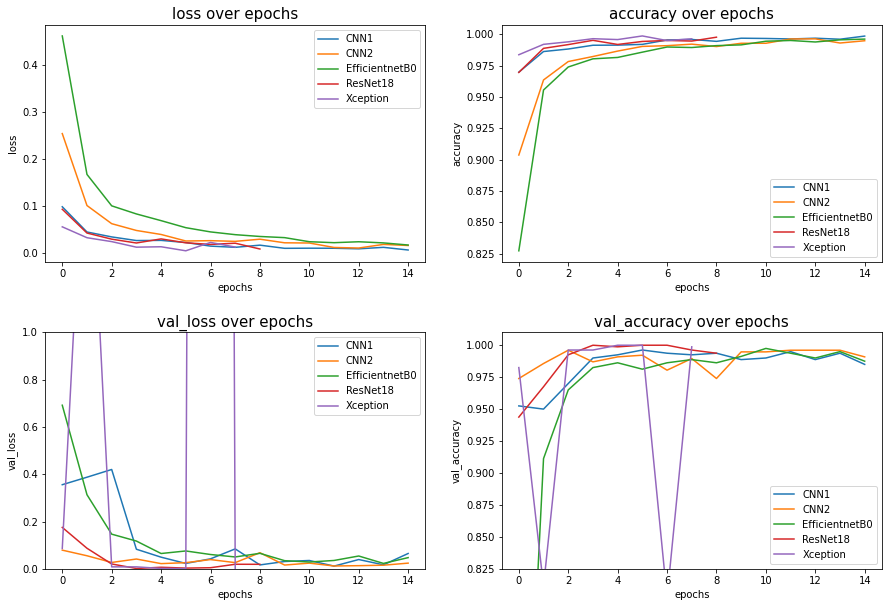
\includegraphics[width=3.6in]{performance_5.png}
\caption{Showing the accuracy and loss in training and validation over epochs}
\label{bench}
\end{figure}

It is interesting to notice that Xception transfer model had lot of fluctations in the accuracy and loss of validation set. That was a symptom of overfitting and could be further reduced by adding better regularization. 

\subsection{Performance on Various Architectures}
In Talbe \ref{tab:2} we list the accuracy and performance benchmarks of the different architectures. It is interesting to notice that for this specific task, increasing the number of parameters had not a huge impact on accuracy, because we can see how a 6.5 million parameter model (Hand-craft1) had almost the same performance of a 22.3 million one (Xception)


% ==================
% # Conclusion #
% ==================
\section{Conclusion}
In conformity with the experimental results, the dataset seems well prepared  as a consequence all the models performed accurately and achieved over 99\% both in accuracy and F1-score. Specifically, the MobilenetV2 model with pre-trained weight can result in the best performance over the other models in terms of accuracy and F1-score. Moreover, compared to other pre-trained models achieving similar accuracy including MnasNet or EfficientNetB0, MobilenetV2 is considerably much more smaller in the number of parameters as such is noticeably applicable to be implemented on any devices specifically edge or mobile as the MobilenetV2 originally designated for with competitive accuracy. However, the simple model of CNNs, such as hand-craft CNN1, provides simple architecture, less complexity with high accuracy as well.

Further developments can be done, such as testing the model with a video live source. In this case it can be useful to use first a segmentation model in order to detect faces in a photo frame and then use our models to detect if a person is wearing a mask or not. 

% ==================
% # Acknowledgment #
% ==================
% use section* for acknowledgment
\section*{Acknowledgment}

The face mask dataset was created by Ashish Jangra (\url{https://www.kaggle.com/ashishjangra27/face-mask-12k-images-dataset}) which consists of almost 12,000 images from google search and the CelebFace dataset created by Jessica Li (\url{https://www.kaggle.com/jessicali9530}). 

In this project we implement the deep learning models using TensorFlow, Keras, and PyTorch. We appreciate all developers involved in those open-source projects. 


% ==============
% # REFERENCES #
% ==============

\printbibliography

\end{document}